\documentclass[aspectratio=169,mathserif]{beamer}
\usepackage{kotex}
\setmainhangulfont{Noto Serif CJK KR}[
  UprightFont=* Light, BoldFont=* Bold,
  Script=Hangul, Language=Korean, AutoFakeSlant,
]
\setsanshangulfont{Noto Sans CJK KR}[
  UprightFont=* DemiLight, BoldFont=* Medium,
  Script=Hangul, Language=Korean, AutoFakeSlant,
]
\setmathhangulfont{Noto Sans CJK KR}[
  SizeFeatures={
    {Size=-6,  Font=* Medium},
    {Size=6-9, Font=*},
    {Size=9-,  Font=* DemiLight},
  },
  Script=Hangul, Language=Korean
]
\usepackage[most]{tcolorbox}
\usepackage{hyperref}
\usepackage{xcolor}
\usepackage{tikz}
\usepackage{graphicx}
\usepackage{amsmath}
\usepackage{amssymb}
\usepackage{caption}
\usepackage{subcaption}
\usepackage{pdftexcmds}
\usepackage{standalone}
\usepackage{ifthen}
\usetikzlibrary{arrows.meta,positioning,calc,fit,backgrounds,shapes.geometric}

\makeatletter
\newcommand{\includegraphviz}[2][]{%
  \typeout{(#2.dot)}%
  \@addtofilelist{#2.dot}%
  \edef\gv@dot{\pdf@filemoddate{#2.dot}}%
  \edef\gv@pdf{\pdf@filemoddate{#2.pdf}}%
  % \pdf@filemoddate returns "" for a missing file, which sorts as "older",
  % so a missing PDF also triggers regeneration
  \ifnum\pdf@strcmp{\gv@dot}{\gv@pdf}>0\relax
    \immediate\write18{dot -Tpdf -Gmargin=0 -o "#2.pdf" "#2.dot"}%
  \fi
  \IfFileExists{#2.pdf}%
    {\includegraphics[#1]{#2.pdf}}%
    {\fbox{Missing #2.pdf — compile with shell-escape enabled}}%
}
\makeatother

\title{MLSys 2026 Google Competition 참가 후기}
\author{데이터플랫폼팀 병장 손량}

\usetheme{default}
\setbeamertemplate{itemize items}[circle]

\AtBeginSection[]
{
\begin{frame}
  \frametitle{Outline}
  \tableofcontents[currentsection]
\end{frame}
}

\begin{document}
\begin{frame}
\maketitle
\end{frame}

\begin{frame}
\frametitle{Outline}
\tableofcontents
\end{frame}

\section{TL;DR}
\begin{frame}{TL;DR}
\framesubtitle{N줄 요약}
\begin{itemize}
  \item MLSys 학회의 대회 트랙에서 구글이 개최한 그래프 스케줄링 대회에 참가했습니다.
  \begin{itemize}
    \item MLSys는 machine learning system을 주제로 하는 국제 학회입니다.
    \item 목표: 계산 그래프의 최적화 알고리즘을 설계하여 NPU에서 최적의 성능을 달성합니다.
    \item 최근 중요도가 높은 머신러닝 시스템의 최적화와 밀접한 관련이 있습니다.
  \end{itemize}
  \pause
  \item 2개월 동안 열심히 연구하고 구현한 끝에 \textbf{최종 3등}을 달성했습니다.
\end{itemize}

\begin{figure}
  \centering
  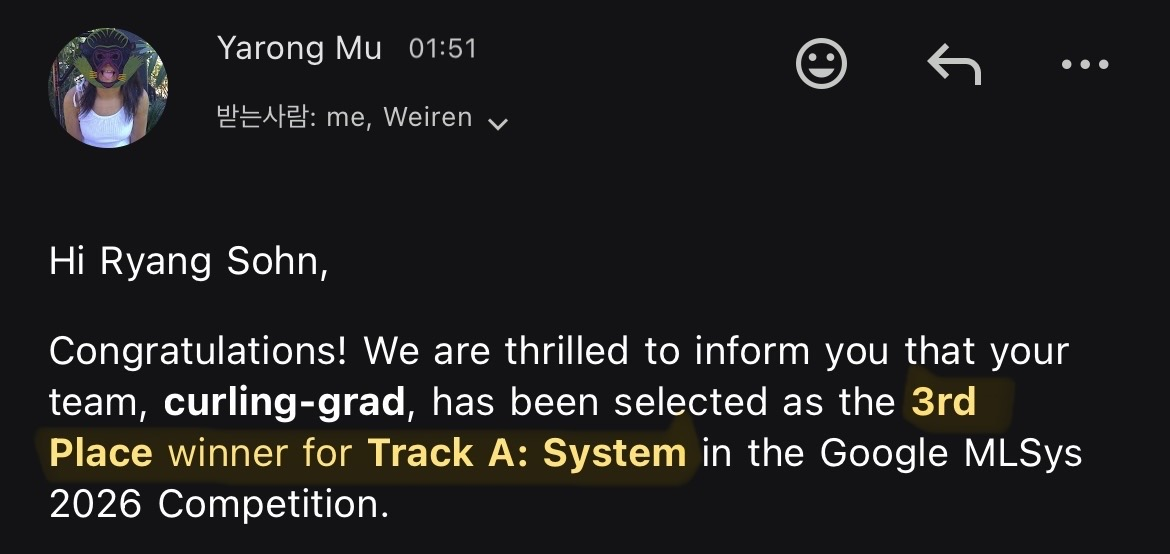
\includegraphics[width=0.5\linewidth]{images/result-email.jpeg}
\end{figure}
\end{frame}

\section{Backround}

\subsection{Systems View on Deep Learning Models}
\begin{frame}{Systems View on Deep Learning Models}
\framesubtitle{딥러닝 모델도 프로그램이다}

\begin{itemize}
  \item CNN, RNN, Transformer 등 딥러닝 모델의 구조는 다양한 종류가 있습니다.
  \item 딥러닝 모델은 다양한 구조를 가지지만, 중요한 특성을 공유합니다.
  \begin{itemize}
    \item \textbf{텐서 연산}으로 이루어져 있습니다.
    \item 전체적인 control flow가 대부분 한 방향만을 따라갑니다.
  \end{itemize}
  \pause
  \item 텐서: \only<2>{\(T: \underbrace{V^* \times \dots \times V^*}_{p\; \text{times}} \times \underbrace{V \times \dots \times V}_{q\; \text{times}} \to \mathbb{R}\) where \(V\) is a vector space ...}\only<3->{다차원 배열}
\end{itemize}
\only<4->{
\begin{figure}
  \centering
  \begin{subfigure}[c]{0.2\textwidth}
    {\resizebox{\linewidth}{!}{\definecolor{cA}{RGB}{66,133,244}
\definecolor{cB}{RGB}{234,67,53}
\definecolor{cC}{RGB}{52,168,83}
\definecolor{cGray}{RGB}{120,120,120}

\begin{tikzpicture}[
  font=\small,
  lbl/.style={font=\footnotesize\itshape},
  op/.style={font=\large},
]
  % ===== Geometry =====
  % cell = 0.3 units.
  % C: cols x 2.3..4.1 (6 cols), rows y 1.0..2.8 (6 rows)
  % Highlighted row: y 1.9..2.2 (4th row). Highlighted col: x 3.2..3.5 (4th col).
 
  % --- A: M x K, 2 cols, 6 rows. x 1.0..1.6 (2 cols), y 1.0..2.8 ---
  \draw[fill=cA!25,draw=cA] (1.0,1.0) rectangle (1.6,2.8);
  \draw[fill=cA!70,draw=cA] (1.0,1.9) rectangle (1.6,2.2);              % highlighted row
  \foreach \y in {1.3,1.6,1.9,2.2,2.5}{\draw[cA!60] (1.0,\y)--(1.6,\y);}
  \draw[cA!60] (1.3,1.0)--(1.3,2.8);                                   % 1 internal vertical
  \draw[cA] (1.0,1.0) rectangle (1.6,2.8);
  \node[lbl] at (1.3,0.65) {$A \in \mathbb{R}^{M \times K}$};
 
  % --- B: K x N, 2 rows, 6 cols. x 2.3..4.1, y 2.95..3.55 ---
  \draw[fill=cB!25,draw=cB] (2.3,2.95) rectangle (4.1,3.55);
  \draw[fill=cB!70,draw=cB] (3.2,2.95) rectangle (3.5,3.55);            % highlighted col
  \foreach \x in {2.6,2.9,3.2,3.5,3.8}{\draw[cB!60] (\x,2.95)--(\x,3.55);}
  \draw[cB!60] (2.3,3.25)--(4.1,3.25);                                 % 1 internal horizontal
  \draw[cB] (2.3,2.95) rectangle (4.1,3.55);
  \node[lbl,anchor=east] at (2.25,3.25) {$B \in \mathbb{R}^{K \times N}$};
 
  % --- C: M x N, 6 cols, 6 rows. x 2.3..4.1, y 1.0..2.8 ---
  \draw[fill=cC!25,draw=cC] (2.3,1.0) rectangle (4.1,2.8);
  \draw[fill=cC!80,draw=cC] (3.2,1.9) rectangle (3.5,2.2);             % output cell
  \foreach \x in {2.6,2.9,3.2,3.5,3.8}{\draw[cC!55] (\x,1.0)--(\x,2.8);}
  \foreach \y in {1.3,1.6,1.9,2.2,2.5}{\draw[cC!55] (2.3,\y)--(4.1,\y);}
  \draw[cC] (2.3,1.0) rectangle (4.1,2.8);
  \node[lbl] at (3.2,0.65) {$C \in \mathbb{R}^{M \times N}$};
 
  % arrows: A-row -> C-cell ; B-col -> C-cell
  \draw[-{Latex},cGray,thick] (1.6,2.05) -- (3.18,2.05);
  \draw[-{Latex},cGray,thick] (3.35,2.95) -- (3.35,2.22);
 
  % ===== Title =====
  \node[op] at (2.25, 4.05) {Matrix Multiplication};
 
  % ===== Normalize height for side-by-side placement =====
  \coordinate (Lx) at (current bounding box.west);
  \coordinate (Rx) at (current bounding box.east);
  \useasboundingbox (Lx |- 0,-0.2476) rectangle (Rx |- 0,4.7045);
\end{tikzpicture}}}
  \end{subfigure}%
  \begin{subfigure}[c]{0.3\textwidth}
    {\resizebox{\linewidth}{!}{\definecolor{cA}{RGB}{66,133,244}
\definecolor{cC}{RGB}{52,168,83}
\definecolor{cGray}{RGB}{120,120,120}

\begin{tikzpicture}[
  font=\small,
  lbl/.style={font=\footnotesize\itshape},
  op/.style={font=\large},
]
  % ---- grid drawing helper (3x3) ----
  \def\grid#1#2#3{% x y color
    \begin{scope}[shift={(#1,#2)}]
      \draw[fill=#3!22,draw=#3,thick] (0,0) rectangle (1.5,1.5);
      \foreach \k in {0.5,1.0}{
        \draw[#3!55] (\k,0)--(\k,1.5);
        \draw[#3!55] (0,\k)--(1.5,\k);}
    \end{scope}}
 
  % ===== Title & definition (centered on rendered image) =====
  \node[op]            at (2.889, 4.55) {Elementwise};
  \node[font=\footnotesize] at (2.889, 3.95) {$B = f(A_1, A_2, \dots, A_k)$};
 
  % ===== Operands: overlapping stacked squares =====
  % A_1 at top-left (back), stack moves down-right to A_k (front, on top)
  \grid{0.30}{2.00}{cA}
  \grid{0.55}{1.75}{cA}
  \grid{0.80}{1.50}{cA}
  % operand list below the stack
  \node[lbl] at (1.30,1.05) {$A_1, \dots, A_k \in \mathbb{R}^{N \times M}$};
 
  % ===== Arrow with f =====
  \draw[-{Latex},cGray,line width=1pt] (2.70,2.50) -- (3.90,2.50)
        node[midway,above,font=\itshape] {$f$};
 
  % ===== Result: single square =====
  \grid{4.30}{1.75}{cC}
  \node[lbl] at (5.05,1.30) {$B \in \mathbb{R}^{N \times M}$};
  %% ===== Normalize height for side-by-side placement =====
  \coordinate (Lx) at (current bounding box.west);
  \coordinate (Rx) at (current bounding box.east);
  \useasboundingbox (Lx |- 0,0.3226) rectangle (Rx |- 0,5.2748);
\end{tikzpicture}}}
  \end{subfigure}%
  \begin{subfigure}[c]{0.25\textwidth}
    {\resizebox{\linewidth}{!}{\definecolor{cA}{RGB}{66,133,244}
\definecolor{cC}{RGB}{52,168,83}
\definecolor{cGray}{RGB}{120,120,120}

\begin{tikzpicture}[
  font=\small,
  lbl/.style={font=\footnotesize\itshape},
  op/.style={font=\large},
]
  % Grids+arrow: A grid [0,1.6] (4x4), arrow, y grid [3.3,3.7] (1x4)
  % cell = 0.4. A: 4 cols x 4 rows. y: 1 col x 4 rows.
  \def\cx{1.9}
 
  % ===== Diagram =====
  % A: 4x4 grid, x 0..2.12, y 0..2.12, cell 0.53
  \begin{scope}[shift={(0.0,0.0)}]
    \draw[fill=cA!25,draw=cA] (0,0) rectangle (2.12,2.12);
    \draw[fill=cA!70,draw=cA] (0,1.06) rectangle (2.12,1.59);       % highlighted row
    \foreach \k in {0.53,1.06,1.59}{\draw[cA!60] (\k,0)--(\k,2.12);}
    \foreach \k in {0.53,1.06,1.59}{\draw[cA!60] (0,\k)--(2.12,\k);}
    \draw[cA] (0,0) rectangle (2.12,2.12);
  \end{scope}
  \node[lbl] at (1.06,-0.35) {$A \in \mathbb{R}^{M \times N}$};
 
  \draw[-{Latex},cGray,thick] (2.52,1.06) -- (3.42,1.06)
        node[midway,above,font=\footnotesize]{$\bigoplus_j$};
 
  % y: 4x1 grid, x 3.82..4.35, y 0..2.12
  \begin{scope}[shift={(3.82,0.0)}]
    \draw[fill=cC!25,draw=cC] (0,0) rectangle (0.53,2.12);
    \draw[fill=cC!80,draw=cC] (0,1.06) rectangle (0.53,1.59);       % highlighted entry
    \foreach \k in {0.53,1.06,1.59}{\draw[cC!60] (0,\k)--(0.53,\k);}
    \draw[cC] (0,0) rectangle (0.53,2.12);
  \end{scope}
  \node[lbl] at (4.085,-0.35) {$y \in \mathbb{R}^{M}$};
 
  % ===== Title & formula on grids+arrow center =====
  \node[op]            at (2.175, 3.05) {Reduction};
  \node[font=\footnotesize] at (2.175, 2.55) {$y_i=\textstyle\bigoplus_j A_{ij}$ (sum/max/\ldots)};
 
  % ===== Equal height + equal top/bottom padding (side-by-side) =====
  \coordinate (Lx) at (current bounding box.west);
  \coordinate (Rx) at (current bounding box.east);
  \useasboundingbox (Lx |- 0,-0.6588) rectangle (Rx |- 0,3.3563);
\end{tikzpicture}}}
  \end{subfigure}%
  \begin{subfigure}[c]{0.175\textwidth}
    {\resizebox{\linewidth}{!}{\definecolor{cA}{RGB}{66,133,244}
\definecolor{cC}{RGB}{52,168,83}
\definecolor{cGray}{RGB}{120,120,120}

\begin{tikzpicture}[
  font=\small,
  lbl/.style={font=\footnotesize\itshape},
  op/.style={font=\large},
]
  % Common vertical center axis
  \def\cx{2.7}
 
  % ===== Title & caption =====
  \node[op]            at (\cx, 2.90) {Reshape};
  \node[font=\footnotesize] at (\cx, 2.40) {same data, new shape};
 
  % source 2x6: 6 cols (width 2.52, center offset 1.05) -> shift_x = cx-1.05
  \begin{scope}[shift={(\cx-1.05,1.85)}]
    \foreach \r in {0,1}{
      \foreach \c in {0,...,5}{
        \pgfmathtruncatemacro{\val}{\r*6+\c+1}
        \node[draw=cA,fill=cA!20,minimum size=0.42cm,inner sep=0pt,font=\tiny]
          at (\c*0.42,-\r*0.42) {\val};}}
  \end{scope}
 
  % arrow (vertical, centered on cx, equal gaps to both grids)
  \draw[-{Latex},cGray,thick] (\cx,1.06) -- (\cx,0.70);
 
  % target 3x4: 4 cols (width 1.68, center offset 0.63) -> shift_x = cx-0.63
  \begin{scope}[shift={(\cx-0.63,0.35)}]
    \foreach \r in {0,1,2}{
      \foreach \c in {0,...,3}{
        \pgfmathtruncatemacro{\val}{\r*4+\c+1}
        \node[draw=cC,fill=cC!20,minimum size=0.42cm,inner sep=0pt,font=\tiny]
          at (\c*0.42,-\r*0.42) {\val};}}
  \end{scope}
  %% ===== Normalize height for side-by-side placement =====
  \coordinate (Lx) at (current bounding box.west);
  \coordinate (Rx) at (current bounding box.east);
  \useasboundingbox (Lx |- 0,-1.2273) rectangle (Rx |- 0,3.7249);
\end{tikzpicture}}}
  \end{subfigure}
\end{figure}}
\end{frame}

\subsection{Computation Graphs}
\begin{frame}{Computation Graphs}
\framesubtitle{Example: Gemma 4 Decoder Block}

\begin{figure}
  \centering
  \resizebox{0.85\textwidth}{!}{%
    \rotatebox{90}{%
      \only<1>{\input{gemma4-decoder/gemma4-decoder}}%
      \only<2>{\input{gemma4-decoder/gemma4-decoder-rmsnorm-highlighted}}%
    }
  }
  \caption{Gemma 4 Decoder Block}
\end{figure}
\end{frame}

\begin{frame}{Computation Graphs}
\framesubtitle{RMSNorm}

RMSNorm의 정의는 다음과 같습니다.
\[
  [\mathrm{RMSNorm}(x)]_i = \frac{x_i w_i}{\sqrt{\mathrm{mean}(x^2) + \epsilon}}
\]
\pause
입력 텐서는 \(x\), \(w\), \(\epsilon\), \(n\)이고, 텐서 연산자와 입력, 출력은 다음과 같이 연결됩니다.
\begin{figure}
  \centering
  \includegraphviz[width=0.9\textwidth]{graphs/rmsnorm}
\end{figure}
\end{frame}

\begin{frame}{Computation Graphs}
\framesubtitle{Example: Gemma 4 Decoder Block}

\begin{figure}
  \centering
  \resizebox{0.85\textwidth}{!}{%
    \rotatebox{90}{%
      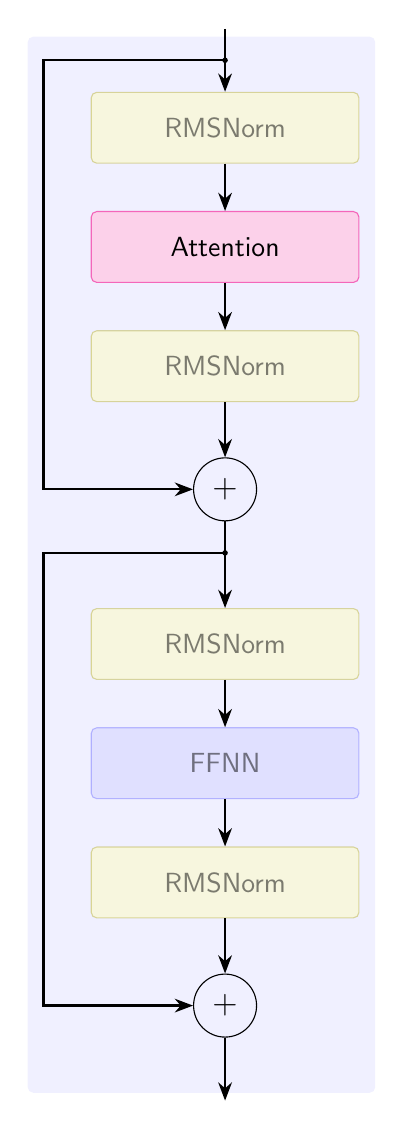
\begin{tikzpicture}[
  font=\sffamily,
  >=Stealth,
  box/.style={rounded corners=2pt,draw,minimum height=9mm,minimum width=34mm,align=center},
  norm/.style={box,fill=yellow!25,draw=olive!60,opacity=0.5,text opacity=0.5},
  global/.style={box,fill=magenta!18,draw=magenta!60,minimum width=34mm,minimum height=9mm},
  ffnn/.style={box,fill=blue!18,draw=blue!50,minimum width=34mm,minimum height=9mm,opacity=0.5,text opacity=0.5},
  add/.style={circle,draw,inner sep=0pt,minimum size=8mm,font=\large},
  line/.style={->,thick}
]

% ---- vertical layout (top to bottom) ----
\node[norm] (n1) {RMSNorm};
\node[global,below=6mm of n1] (attn) {Attention};
\node[norm,below=6mm of attn] (n2) {RMSNorm};
\node[add,below=7mm of n2] (add1) {$+$};

\node[norm,below=11mm of add1] (n3) {RMSNorm};
\node[ffnn,below=6mm of n3] (ffnn) {FFNN};
\node[norm,below=6mm of ffnn] (n4) {RMSNorm};
\node[add,below=7mm of n4] (add2) {$+$};

% ---- main path ----
\draw[line] (n1) -- (attn);
\draw[line] (attn) -- (n2);
\draw[line] (n2) -- (add1);
\draw[line] (add1) -- (n3);
\draw[line] (n3) -- (ffnn);
\draw[line] (ffnn) -- (n4);
\draw[line] (n4) -- (add2);

% ---- input / output stubs ----
\coordinate (in) at ($(n1.north)+(0,8mm)$);
\draw[line] (in) -- (n1.north);
\draw[line] (add2.south) -- ($(add2.south)-(0,8mm)$);

% ---- residual connections (left side) ----
\coordinate (tap1) at ($(in)!0.5!(n1.north)$);
\coordinate (lx) at ($(n1.west)+(-6mm,0)$);
\coordinate (l1) at (lx);
\coordinate (l2) at (lx);
\coordinate (tap2) at ($(add1.south)+(0,-4mm)$);
\draw[line] (tap1) -- (tap1 -| lx) -- (add1.west -| lx) -- (add1.west);
\fill (tap1) circle (1pt);

\draw[line] (tap2) -- (tap2 -| lx) -- (add2.west -| lx) -- (add2.west);
\fill (tap2) circle (1pt);

% ---- enclosing decoder box ----
\begin{scope}[on background layer]
  \node[rounded corners=2pt,fill=blue!6,
        fit=(n1)(attn)(n2)(add1)(n3)(ffnn)(n4)(add2)(l1)(l2),
        inner ysep=7mm,inner xsep=2mm] (dec) {};
\end{scope}

\end{tikzpicture}%
    }
  }
  \caption{Gemma 4 Decoder Block}
\end{figure}
\end{frame}

\begin{frame}{Computation Graphs}
\framesubtitle{Attention}
Attenton의 정의는 다음과 같습니다.
\begin{align*}
  \mathrm{Attention}(Q, K, V) = \mathrm{softmax}\left(\frac{QK^T}{\sqrt{d_k}}\right) V, \quad
  [\mathrm{softmax}(x)]_i = \frac{\exp{(x_i)}}{\sum_i \exp{(x_i)}}
\end{align*}
\pause
입력 텐서는 \(Q\), \(K\), \(V\), \(d_k\)이고, 계산 그래프는 다음과 같습니다.
\begin{figure}
  \centering
  \includegraphviz[width=\textwidth]{graphs/attention}
\end{figure}
\end{frame}

\subsection{Hardware for Deep Learning}
\begin{frame}{Hardware for Deep Learning}
\framesubtitle{Tiled Matmul}

\begin{itemize}
  \item 딥러닝에서 가장 많이 사용되는 연산은 행렬 곱셈입니다.
  \begin{itemize}
    \item 행렬 곱셈을 빠르게 할수록 딥러닝 모델의 실행 속도를 개선할 수 있습니다.
  \end{itemize}
  \item 이렇게 행렬을 타일 단위로 곱하면 여러 이점이 있습니다.
  \begin{enumerate}
    \item 같은 연산을 위해 사용해야 하는 명령어 수를 줄입니다.
    \pause
    \item \textbf{메모리 접근 수를 줄입니다.}
  \end{enumerate}
\end{itemize}
\pause
\begin{figure}
  \centering
  \only<1-3>{%
    \resizebox{0.8\linewidth}{!}{\includestandalone{tiled-matmul/matmul-1x1}}%
    \caption{1x1 원소를 계산하는데 원소 8개, 총 8\texttimes 16 = 128개를 읽어야 합니다.}%
  }
  \only<4>{%
    \resizebox{0.8\linewidth}{!}{\includestandalone{tiled-matmul/matmul-2x2}}%
    \caption{2x2 원소를 계산하는데 원소 16개, 총 16\texttimes 4 = 64개를 읽어야 합니다.}%
  }
\end{figure}
\end{frame}

\begin{frame}{Hardware for Deep Learning}
\framesubtitle{Pipelining}

일반적으로 텐서 연산은 메모리 접근과 연산을 동시에 수행할 수 있습니다.

\begin{figure}
  \centering
  \only<1>{\resizebox{0.9\linewidth}{!}{\includestandalone{pipeline-animation/frame1_parallel}}}%
  \only<2>{\resizebox{0.9\linewidth}{!}{\includestandalone{pipeline-animation/frame2_parallel}}}%
  \only<3>{\resizebox{0.9\linewidth}{!}{\includestandalone{pipeline-animation/frame3_parallel}}}%
  \only<4>{\resizebox{0.9\linewidth}{!}{\includestandalone{pipeline-animation/frame4_parallel}}}%
  \only<5>{\resizebox{0.9\linewidth}{!}{\includestandalone{pipeline-animation/frame5_parallel}}}%
  \only<6>{\resizebox{0.9\linewidth}{!}{\includestandalone{pipeline-animation/frame6_parallel}}}%
  \only<7>{\resizebox{0.9\linewidth}{!}{\includestandalone{pipeline-animation/frame7_parallel}}}%
  \only<8>{\resizebox{0.9\linewidth}{!}{\includestandalone{pipeline-animation/frame8_parallel}}}
\end{figure}
\end{frame}

\begin{frame}{Hardware for Deep Learning}
\framesubtitle{Roofline Model}

\begin{itemize}
  \item 메모리 접근과 연산을 병렬화하면 전체 속도는 둘 중 느린 것에 의해 정해집니다.
  \item 대부분의 하드웨어에서 메모리는 연산 속도보다 느립니다.
  \begin{itemize}
    \item B200 GPU: 2,250 TFLOPS (BF16) vs 8 TB/s
    \item 연산 속도는 더 큰 칩을 만들면 늘릴 수 있지만, 메모리는 빠르게 하기 어렵습니다.
    \item 보통 compute bound가 되는 것을 목표로 최적화합니다.
  \end{itemize}
\end{itemize}

\begin{figure}
  \centering
  \begin{subfigure}{0.5\textwidth}
    \resizebox{!}{2.8cm}{\includestandalone{pipeline-diagrams/compute-bound}}
    \caption{Compute bound}
  \end{subfigure}
  \begin{subfigure}{0.45\textwidth}
    \resizebox{!}{2.8cm}{\includestandalone{pipeline-diagrams/balanced}}
    \caption{Balanced}
  \end{subfigure}
\end{figure}
\end{frame}

\subsection{Operator Fusion}
\begin{frame}{Operator Fusion}
\framesubtitle{Example: Chain of Elementwise Operators}

\begin{figure}
  \centering
  \includegraphviz[width=0.5\linewidth]{graphs/addmul}
  \caption{\((A + B) * C\)의 계산 그래프}
\end{figure}

\begin{itemize}
  \item 덧셈과 곱셈을 따로 실행한다고 가정합시다.
  \begin{itemize}
    \item 덧셈 결과를 메모리에 저장하고 곱셈하기 전에 다시 읽어야 합니다.
    \item 덧셈과 곱셈 연산보다 메모리 접근에 시간이 낭비됩니다.
  \end{itemize}
  \item 덧셈과 곱셈을 한번에 실행하면 낭비되는 시간을 줄일 수 있습니다.
\end{itemize}
\end{frame}

\begin{frame}{Operator Fusion}
\framesubtitle{Example: Chain of Elementwise Operators}

\begin{figure}
  \centering
  \resizebox{\linewidth}{!}{\includestandalone{pipeline-diagrams/fusion-timeline}}
\end{figure}

여전히 memory bound 이지만, 실행 시간이 훨씬 줄었습니다.
\end{frame}

\begin{frame}{Operator Fusion}
\framesubtitle{계산을 더 많이 하고도 빨라질 수 있다?}

\begin{figure}
  \centering
  \includegraphviz[width=0.75\linewidth]{graphs/residual}
  \caption{Residual connection이 있는 그래프}
\end{figure}

\begin{itemize}
  \item op2와 op3를 한번에 계산할 수 없다고 가정합시다.
  \item op1과 op2를 합치면 op3에서 입력을 받을 수 없고, 반대도 마찬가지입니다.
  \pause
  \item op1의 계산량이 적다면, (op1, op2), (op1, op3)로 합치는 것이 빠를 수 있습니다.
  \item FlashAttention과 같은 고성능 커널 설계에 이 아이디어가 이용된 바 있습니다.
\end{itemize}
\end{frame}

\section{Solving the Problem}

\subsection{Problem Analysis}
\begin{frame}{Problem Analysis}

\begin{tcolorbox}[title={문제의 목표}]
  계산 그래프가 주어질 때, 하드웨어에서 빠르게 실행하는 전략을 찾아야 합니다.
\end{tcolorbox}
\pause

\begin{itemize}
  \item 문제에서 가정하는 하드웨어는 일반적인 NPU와 비슷한 구조를 갖고 있습니다.
  \begin{itemize}
    \item 빠르고 공간이 제한된 메모리와 느리고 공간이 큰 두 종류의 메모리가 있습니다.
    \item 계산 그래프를 노드 그룹 단위로, 텐서 연산을 타일 단위로 실행합니다.
    \item 텐서 연산을 위해서는 입력 텐서의 타일을 빠른 메모리로 로드해야 합니다.
    \item 메모리 접근과 계산을 동시에 수행할 수 있습니다.
  \end{itemize}
  \pause
  \item 입력으로 어떤 계산 그래프가 주어질지 알 수 없습니다.
  \begin{itemize}
    \item 특정한 경우에 대해서만 실행 전략을 찾는 것으로는 부족합니다.
    \item 가능한 입력에 대해서 일반적으로 빠른 실행 전략을 찾는 알고리즘을 설계해야 합니다.
  \end{itemize}
\end{itemize}
\end{frame}

\begin{frame}{Problem Analysis}
\framesubtitle{Execution Strategy}

알고리즘은 크게 세 가지 변수에 대한 최적값을 찾아야 합니다.
\begin{enumerate}
  \item 하드웨어에서 한번에 실행할 노드 그룹
  \item 각 그룹에 있는 텐서 연산의 실행 타일 크기
  \item 그룹의 출력 중, 느린 메모리를 거치지 않을 텐서
\end{enumerate}
\end{frame}

\newcommand{\animframe}[1]{\resizebox{\linewidth}{!}{\includestandalone{example3-animation/#1}}}

\begin{frame}{Problem Analysis}
\framesubtitle{Example: Strategy on Residual Connection}

% ----- Colours / styles / drawing macros ONLY (no \usepackage).
% Safe to \input inside a group in the document body, so the names stay scoped.
% ======================================================================
%  tikzcommon.tex  --  Example 3 / Strategy B, software-pipelined view.
%  Each tile interval overlaps load(next) and store(prev) on the single
%  memory channel with compute, so interval = max(load+store, compute).
%  A Gantt strip at the bottom shows the staggering.  Every common element
%  is defined here once -> byte-identical across frames (no \only<> jitter).
% ======================================================================

\newcommand{\CanvasW}{16}
\newcommand{\CanvasH}{9}
\newcommand{\CanvasBB}{\useasboundingbox (-0.35,2.20) rectangle (12.7,7.7);}

% ---- palette ----------------------------------------------------------
\definecolor{ink}{RGB}{34,34,40}
\definecolor{sgA}{RGB}{37,99,235}     % subgraph 0 / compute A,B (blue)
\definecolor{sgB}{RGB}{234,88,12}     % subgraph 1 / compute C,D (orange)
\definecolor{resG}{RGB}{22,163,74}    % resident / retained (green)
\definecolor{inB}{RGB}{59,130,246}    % load  (blue)
\definecolor{outO}{RGB}{217,70,12}    % store (orange)
\definecolor{play}{RGB}{222,30,30}    % playhead cursor (red)
\definecolor{panel}{RGB}{205,208,214}
\definecolor{soft}{RGB}{246,247,249}
\definecolor{ttl}{RGB}{20,20,26}

\tikzset{
  opnode/.style ={circle,draw=ink,line width=0.9pt,fill=soft,
                  minimum size=0.82cm,inner sep=0pt,font=\small\bfseries},
  ionode/.style ={rectangle,draw=ink,line width=0.9pt,
                  fill=soft,minimum size=0.76cm,inner sep=1pt,font=\small\bfseries},
  tedge/.style  ={-{Latex[length=2.0mm]},draw=ink!75,line width=0.9pt},
  tlab/.style   ={font=\scriptsize,text=ink!65,inner sep=1pt},
  outframe/.style={draw=panel,line width=1pt},
}

% ---- output-map cells (map (7.4,5.4)-(9.1,7.1), split y=6.25) ---------
\newcommand{\tilefill}[2]{%
  \ifthenelse{\equal{#1}{top}}{\fill[#2!35] (7.4,6.25) rectangle (9.1,7.1);}{}%
  \ifthenelse{\equal{#1}{bot}}{\fill[#2!35] (7.4,5.4)  rectangle (9.1,6.25);}{}%
  \ifthenelse{\equal{#1}{both}}{\fill[#2!28] (7.4,5.4) rectangle (9.1,7.1);}{}%
}
\newcommand{\activeborder}[2]{%
  \ifthenelse{\equal{#1}{top}}%
    {\draw[#2,dash pattern=on 2.5pt off 2pt,line width=1.2pt] (7.46,6.31) rectangle (9.04,7.04);}{}%
  \ifthenelse{\equal{#1}{bot}}%
    {\draw[#2,dash pattern=on 2.5pt off 2pt,line width=1.2pt] (7.46,5.46) rectangle (9.04,6.19);}{}%
}

% ---- subgraph halos ---------------------------------------------------
% op1 (2.3,5.3) -- op2 (3.7,6.7): 45-deg axis, midpoint (3.0,6.0).
% Rectangle is centred on the midpoint then rotated about it, so it hugs
% exactly the two nodes (half-length 1.58 along axis, half-width 0.59).
\newcommand{\haloSGzero}[2]{%
  \begin{scope}[opacity=#1]
    \begin{scope}[rotate around={45:(3.0,6.0)}]
      \fill[sgA!30] (1.42,5.41) rectangle (4.58,6.59);
    \end{scope}
  \end{scope}
  \ifnum#2=1\node[font=\scriptsize\bfseries,text=sgA] at (1.95,6.98){Subgraph 0};\fi}
\newcommand{\haloSGone}[2]{%
  \begin{scope}[opacity=#1]\fill[sgB!35] (1.78,4.74) rectangle (5.30,5.86);\end{scope}
  \ifnum#2=1\node[font=\scriptsize\bfseries,text=sgB] at (4.55,4.55){Subgraph 1};\fi}

\newcommand{\sinkring}[3]{\draw[line width=1.7pt,#3] (#1,#2) circle (0.52);}
\newcommand{\recomputeTag}{%
  \node[font=\scriptsize,text=sgB] at (2.3,4.40){$\circlearrowleft$ recompute op1};
  \draw[sgB,-{Latex[length=1.6mm]},line width=0.8pt] (2.3,4.57)--(2.3,4.80);}

\newcommand{\tilemark}[1]{% #1 = formatted tensor label, e.g. $T_2$ or out
  \node[font=\scriptsize,text=ink] at (8.25,6.675){#1:t};
  \node[font=\scriptsize,text=ink] at (8.25,5.825){#1:b};}
\newcommand{\memtext}[2]{%
  \node[anchor=north west,font=\scriptsize,text=ink] at (7.4,5.18){\textbf{Fast memory:}\; #1};
  \node[anchor=north west,font=\scriptsize,text=ink] at (7.4,4.80){\textbf{Slow memory:}\; #2};}

% ======================================================================
%  Pipeline Gantt strip.  \pipe{active}  active: -1 init, 0..5 cols, 6 done
%  columns: 0 fill(ld A) | 1 K_A(ld B) | 2 K_B(ld C) | 3 K_C(ld D)
%           | 4 K_D(st C) | 5 drain(st D)
% ======================================================================
\newcommand{\pipe}[1]{% #1 = playhead x (time). <1.5 hides bar/fades all; >12.3 all solid.
  \node[font=\scriptsize\bfseries,text=ink!80,anchor=east] at (1.40,3.70){Compute};
  \node[font=\scriptsize\bfseries,text=ink!80,anchor=east] at (1.40,2.85){Memory};
  \foreach \gx in {3.3,5.1,6.9,8.7,10.5}{%
    \draw[black!16,line width=0.4pt,dash pattern=on 1.6pt off 1.6pt] (\gx,2.51)--(\gx,4.04);}
  % MEMORY channel (packed, bottleneck)
  \foreach \xL/\xR/\ml/\mc in {%
      1.5/3.3/{ld $A$:t}/inB, 3.3/5.1/{ld $A$:b}/inB,
      5.1/6.9/{ld $A$:t}/inB, 6.9/8.7/{ld $A$:b}/inB,
      8.7/10.5/{st out:t}/outO, 10.5/12.3/{st out:b}/outO}{%
    \pgfmathparse{\xL>#1 ? 0.18 : 1.0}\edef\om{\pgfmathresult}%
    \begin{scope}[opacity=\om]
      \fill[\mc!18] (\xL,2.55) rectangle (\xR,3.15);
      \draw[\mc,line width=0.7pt] (\xL,2.55) rectangle (\xR,3.15);
      \node[font=\tiny,text=ink] at ({(\xL+\xR)/2},2.85){\ml};
    \end{scope}}%
  % COMPUTE op steps: each tile after its load lands
  \foreach \xL/\opa/\opb/\cc in {%
      3.3/op1/op2/sgA, 5.1/op1/op2/sgA, 6.9/op1/op3/sgB, 8.7/op1/op3/sgB}{%
    \pgfmathparse{\xL>#1 ? 0.18 : 1.0}\edef\oA{\pgfmathresult}%
    \begin{scope}[opacity=\oA]
      \fill[\cc!22] (\xL,3.40) rectangle ({\xL+0.439},4.00);
      \draw[\cc,line width=0.7pt] (\xL,3.40) rectangle ({\xL+0.439},4.00);
      \node[font=\tiny,text=ink] at ({\xL+0.22},3.70){\opa};
    \end{scope}
    \pgfmathparse{(\xL+0.439)>#1 ? 0.18 : 1.0}\edef\oB{\pgfmathresult}%
    \begin{scope}[opacity=\oB]
      \fill[\cc!22] ({\xL+0.439},3.40) rectangle ({\xL+0.878},4.00);
      \draw[\cc,line width=0.7pt] ({\xL+0.439},3.40) rectangle ({\xL+0.878},4.00);
      \node[font=\tiny,text=ink] at ({\xL+0.659},3.70){\opb};
    \end{scope}}%
  % PLAYHEAD: vertical cursor at current time
  \pgfmathparse{(#1>=1.5)&&(#1<=12.3) ? 1 : 0}\edef\showbar{\pgfmathresult}%
  \ifdim\showbar pt>0.5pt
    \draw[play,line width=0.6pt,dash pattern=on 2.4pt off 1.8pt] (#1,2.40)--(#1,4.15);
  \fi
}

% ======================================================================
\newcommand{\StaticScene}{%
  % graph
  \node[ionode] (A)   at (1.0,5.3){$A$};
  \node[opnode] (op1) at (2.3,5.3){op1};
  \node[opnode] (op2) at (3.7,6.7){op2};
  \node[opnode] (op3) at (4.7,5.3){op3};
  \node[ionode] (out) at (6.0,5.3){out};
  \draw[tedge] (A)--(op1); \draw[tedge] (op1)--(op2);
  \draw[tedge] (op1)--(op3); \draw[tedge] (op2)--(op3); \draw[tedge] (op3)--(out);
  \node[tlab] at (2.78,6.05){$T_1$};
  \node[tlab] at (3.50,5.08){$T_1$};
  \node[tlab] at (4.42,6.05){$T_2$};
  % output map
  \draw[outframe] (7.4,5.4) rectangle (9.1,7.1);
  \draw[panel,line width=1pt] (7.4,6.25)--(9.1,6.25);
}

\begin{figure}
\centering
  \only<1>{\resizebox{\linewidth}{!}{\animframe{frame0}}}%
  \only<2>{\resizebox{\linewidth}{!}{\animframe{frame1}}}%
  \only<3>{\resizebox{\linewidth}{!}{\animframe{frame2}}}%
  \only<4>{\resizebox{\linewidth}{!}{\animframe{frame3}}}%
  \only<5>{\resizebox{\linewidth}{!}{\animframe{frame4}}}%
  \only<6>{\resizebox{\linewidth}{!}{\animframe{frame5}}}%
  \only<7>{\resizebox{\linewidth}{!}{\animframe{frame6}}}%
  \only<8>{\resizebox{\linewidth}{!}{\animframe{frame7}}}%
  \only<9>{\resizebox{\linewidth}{!}{\animframe{frame8}}}%
  \only<10>{\resizebox{\linewidth}{!}{\animframe{frame9}}}%
  \only<11>{\resizebox{\linewidth}{!}{\animframe{frame10}}}%
  \only<12>{\resizebox{\linewidth}{!}{\animframe{frame11}}}
\end{figure}
\end{frame}

\begin{frame}{Problem Analysis}
\framesubtitle{이거 웰노운 아닌가?}

\begin{itemize}
  \item 결국 문제의 핵심은 operator fusion을 잘하는 것입니다.
  \begin{itemize}
    \item Operator fusion은 머신러닝 시스템 분야에서 활발히 연구되고 있는 주제입니다.
    \item PyTorch, JAX, TensorRT 등 다양한 런타임에 구현되어 있습니다.
    \item ``코딩할 시간도 얼마 없는데 이미 잘 구현된 아이디어를 참고하면 되지 않을까?''
  \end{itemize}
  \pause
  \item 대부분의 런타임에서 operator fusion은 rule based 기법으로 구현합니다.
  \begin{itemize}
    \item 자주 나타나는 패턴과 최적화 방식을 미리 입력해 두고, 패턴 매칭을 통해 최적화합니다.
    \item 예시: 행렬 곱의 결과를 ReLU가 사용하는 경우, 두 연산을 함께 실행합니다.
  \end{itemize}
\end{itemize}

\pause
\begin{figure}
  \centering
  \only<1-3>{\resizebox{!}{2.5cm}{\includegraphviz[width=\linewidth]{graphs/nn-twolayer}}}%
  \only<4>{\resizebox{!}{2.5cm}{\includegraphviz[width=\linewidth]{graphs/nn-twolayer-fused}}}
\end{figure}
\end{frame}

\begin{frame}{Problem Analysis}
\framesubtitle{날로 먹기란 쉽지 않다}

\begin{itemize}
  \item Rule based 기법을 적용하려면 패턴을 그래프에서 찾기 쉬워야 합니다.
  \begin{itemize}
    \item 일반적인 그래프는 행렬 곱, ReLU, reshape 등 다양한 종류의 연산이 있습니다.
    \pause
    \item 하지만 이 문제의 그래프에서는 연산 종류가 matmul, elementwise 두 종류뿐입니다.
    \item 원래는 연산 종류로 실행 시간을 예상할 수 있지만, 문제에서는 임의로 주어집니다.
  \end{itemize}
\end{itemize}

\pause
\begin{figure}
  \centering
  \includegraphviz[width=0.9\linewidth]{graphs/arbitrary-cost}
\end{figure}

\pause
\begin{tcolorbox}[title={전체적인 전략}]
  패턴 매칭 대신, 다양한 최적화 전략을 탐색하는 알고리즘을 구현해야 합니다.
\end{tcolorbox}
\end{frame}

\subsection{Global Optimization}
\begin{frame}{Global Optimization}
\framesubtitle{Defining the Search Space}

\begin{itemize}
  \item Operator fusion 탐색 공간은 매우 방대합니다.
  \begin{itemize}
    \item 탐색 공간이 계산 그래프의 연산자 개수에 대해 지수적으로 늘어납니다.
    \item ``무식하게'' 탐색하면 \only<1>{전역하기 전까지 답을 못 구할수도 있습니다.}\only<2->{지구가 멸망하기 전까지 답을 못 구할수도 있습니다.}
  \end{itemize}
\end{itemize}

\pause
\begin{tcolorbox}[title={탐색 공간의 정의}]
  효율적으로 탐색하되 최적에 가까운 답을 구할 수 있도록 공간을 정의해야 합니다.
\end{tcolorbox}

\pause
\begin{itemize}
  \item 탐색 공간 정의도 operator fusion에서 중요하기 때문에 다양한 연구가 있습니다.
  \item Optimal Kernel Orchestration for Tensor Programs with Korch (ASPLOS '24)
  \begin{itemize}
    \item 간단한 operator fusion 외의 다양한 패턴도 효율적으로 탐색할 수 있습니다.
  \end{itemize}
\end{itemize}
\end{frame}

\begin{frame}{Global Optimization}
\framesubtitle{Taming the Search Space}

\begin{itemize}
  \item \(N\)개 연산자가 있을 때 동시에 실행할 수 있는 그룹은 \(2^N\)개입니다.
  \begin{itemize}
    \item 각 연산자마다 동시에 실행할 그룹에 있음/없음 2가지 경우가 가능하기 때문입니다.
  \end{itemize}
  \pause
  \item 이 \(2^N\)개 모두를 고려할 필요는 없다는 사실에 주목해야 합니다.
\end{itemize}
\pause
\begin{figure}
  \centering
  \includegraphviz[width=0.8\linewidth]{graphs/bad-fusion}
\end{figure}
\begin{itemize}
  \item Korch에서는 의미 있는 경우만 탐색하기 위해 convex subgraph를 사용합니다.
  \begin{itemize}
    \item Convex subgraph만을 고려하면 개수가 \(2^N\)개에서 \(N^2\)개에 가깝게 줄어듭니다.
    \item 이 후보들 중 BLP(Binary Linear Programming)을 통해 실행할 그룹을 결정합니다.
  \end{itemize}
\end{itemize}
\end{frame}

\begin{frame}{Global Optimization}
\framesubtitle{Taming the Search Space}

\begin{tcolorbox}[title={Convex subgraph의 정의}]
  그래프 \(G = (V, E)\)에 대해, 노드 집합 \(V\,'\subset V\)는 모든 노드 쌍 \(v_1, v_2 \in V\,'\)에 대해 \((v_1, u), (u, v_2) \in E\)인 \(u \in V \setminus V\,'\)이 존재하지 않을 때 \(G\)의 convex subgraph를 형성합니다.
\end{tcolorbox}
\end{frame}

\subsection{Local Optimization}
\begin{frame}{Local Optimization}
\framesubtitle{Choosing Retained Tensors}

\begin{itemize}
  \item 그룹의 텐서를 느린 메모리를 거치지 않도록 지정할 수 있습니다.
  \begin{itemize}
    \item 빠른 메모리 공간을 차지하기 때문에, 꼭 필요한 텐서만을 선택해야 합니다.
  \end{itemize}
  \item Operator fusion과 같이, 무식하게 모든 경우를 탐색할 수는 없습니다.
\end{itemize}
\pause
\begin{figure}
  \centering
  \only<1-2>{\includegraphviz[width=0.8\linewidth]{graphs/bad-retention}}%
  \only<3->{\includegraphviz[width=0.8\linewidth]{graphs/good-retention}}
\end{figure}
\pause
\begin{tcolorbox}[title={제약 조건}]
  빠른 메모리에 유지할 텐서는 그룹의 경계에 있어야 의미가 있습니다.
\end{tcolorbox}
\end{frame}

\begin{frame}{Local Optimization}
\framesubtitle{Partitioning Graphs}

\begin{itemize}
  \item 추가적으로, 유지되는 텐서는 최대 한 개의 그룹에서만 사용 가능합니다.
  \item 이 관점에서, 유지되는 텐서를 선택하는 것은 선택된 그룹의 분할 문제와 같습니다.
\end{itemize}
\pause
\begin{figure}
  \centering
  \only<1-2>{\resizebox{!}{2.5cm}{\includegraphviz[width=\linewidth]{graphs/before-retention}}}%
  \only<3->{\resizebox{!}{2.5cm}{\includegraphviz[width=\linewidth]{graphs/after-retention}}}
\end{figure}
\pause
\begin{itemize}
  \item 실행 그룹의 각 텐서들에 대해 유지 여부를 결정해 추가적인 최적화를 구현했습니다.
\end{itemize}
\end{frame}

\section{Meta-strategy}
\begin{frame}{Meta-strategy}
\framesubtitle{군대에서 대회하기}

\begin{itemize}
  \item 가장 큰 어려움: 시간이 매우 부족합니다.
  \begin{itemize}
    \item 파견 전이었기 때문에 물리적으로 키보드를 잡을 시간이 절대적으로 없습니다.
    \item 불행 중 다행히 남는 일과시간을 논문을 읽고 설계하는데 쓸 수 있었습니다.
    \item 사지방에서 논문 프린트 \textrightarrow{} 남는 일과시간에 읽기, 설계 \textrightarrow{} 사지방에서 구현
  \end{itemize}
  \pause
  \item LLM은 확실히 Rust를 짤 때 오류가 적습니다.
  \begin{itemize}
    \item 순수 재미를 위해 Rust를 구현 언어로 선택했지만, 의외로 도움이 되었습니다.
    \item 의도가 코드에 명확하게 나타나고, 성능이 보장되면서 컴파일러가 오류를 잡아줍니다.
    \item LLM의 약점인 논리적 사고를 컴파일러가 대신 해 줄 수 있습니다.
  \end{itemize}
  \pause
  \item 아 이거 좋을것같은데 \textrightarrow{} 누군가 이미 했습니다.
  \begin{itemize}
    \item 특히 operator fusion 같은 유명한 주제는 많은 연구가 진행되어 있습니다.
    \item 선행 연구를 찾다가 아이디어를 얻을 때가 많이 있었습니다.
    \item 하지만 논문도 오류가 있을 수 있기 때문에 구현할 때 유의해야 합니다.
  \end{itemize}
\end{itemize}
\end{frame}

\begin{frame}
\frametitle{Thank You!}

코드와 발표 자료 등은 깃헙 저장소에서 확인할 수 있습니다.

\url{https://github.com/sohnryang/mlsys2026-graph-scheduling}
\end{frame}
\end{document}